\documentclass{utmthesis}
\usepackage{graphicx}
\usepackage{url} 
\usepackage[pages=some]{background}
\usepackage{natbib}
\usepackage{multirow}
\usepackage{subfig}
\usepackage{amsmath}
\usepackage{amssymb}
\usepackage{tabulary}
\usepackage{algorithm}
\usepackage{algpseudocode}
\captionsetup{belowskip=12pt,aboveskip=4pt}
\begin{document}

% Required information
\title{Algorithm Selection for Subgraph Isomorphism Problems:}
\titletwo{A Reinforcement Learning Approach}
\author{Paul Kenneth Valdez Rigor}
\degree{Masters of Science}
\specialization{Computer Science}
\intakeyear{2018}
\faculty{Faculty of Computing}
\titledate{October 2018}
\award{3}
% Options for Award 
% 1. Bachelor Degree Project Report
% 2. Master's Project Report (By course work)
% 3. Master's Dissertation (By course work and research)
% 4. Master's Thesis (By research)
% 5. Doctor of Philosophy Thesis
% 6. Other PhD Thesis
% 7. Generic PhD Thesis
% 8. Thesis Proposal
\superone{Assoc. Prof. Dr. Roliana Binti Ibrahim}
\supertwo{Dr. Haza Nuzly Abdull Hamed}

% Option for two-page printing
\newgeometry{top=2.5cm,left=4cm,right=2.5cm,bottom=2.5cm,twoside}

% Option to add watermark page
% Comment for final version	
\backgroundsetup{scale=1,angle=0,opacity=.1,hshift=0.25in,vshift=-0.5in,contents={
\includegraphics[width=5cm]{img/utm02.jpg}}}
\watermarkpage

% Mandatory pages
\coverpage
\superpage
\certification
\frontmatter
\maketitle
\declaration

\begin{abstract}
A set of hard computational problems can be solved more efficiently when using multiple algorithms instead of a single algorithm. This technique is called algorithm selection. An algorithm selection model captures the relationship between problem features and algorithm performance, using this knowledge to assign the best-performing algorithms to problems. Most approaches in literature use supervised learning techniques to learn the problem feature–algorithm performance relationship. This study presents a different perspective by training algorithm selection models using reinforcement learning---an experience-driven learning approach inspired by how humans and animals naturally learn from their environment. REINFORCE, the proposed reinforcement learning algorithm, is compared with pairwise random forest regression, a supervised learning algorithm from a previously related study. Experiment results show that an algorithm selection model trained using REINFORCE performs poorly as compared to one trained using pairwise random forest regression. However, zooming into the results reveal that REINFORCE did better than pairwise random forest regression on solving the easier problems, which constitutes the majority of the dataset. Still, REINFORCE fails because it is not able to perform well on solving the much harder problems on the dataset, which have a huge impact on the final calculation of algorithm selection performance scores. Nevertheless, this study maintains hope on the potential of reinforcement learning in producing algorithm selection models with better performance than models trained using supervised learning techniques. 
\end{abstract}

\tableofcontents
\listoftables
\listoffigures

%List of abbreviation 
\listofabbre
\addabbre{AS}{Algorithm Selection}
\addabbre{ASlib}{Algorithm Selection Library}
\addabbre{COSEAL}{Configuration and Selection of Algorithms}
\addabbre{MCP}{Misclassification Penalty}
\addabbre{PRFR}{Pairwise random forest regression}
\addabbre{RL}{Reinforcement Learning}
\addabbre{SBS}{Single Best Solver}
\addabbre{SAT}{Satisfiability}
\addabbre{VBS}{Virtual Best Solver}
\addabbre{TSP}{Travelling Salesman Problem}
\addabbre{PORTSUB}{Paper by \citet{kotthoff2016portfolios}}
\addabbre{REINFORCE}{REward INcrement = Nonnegative Factor + Offset Reinforcement + Characteristic Eligibility}
\addabbre{LLAMA}{Leveraging Learning to Automatically Manage Algorithms}

\onehalfspacing
\mainmatter

% You can call another LaTeX document 
\chapter{Introduction}
\section{Introduction}
The \textit{algorithm selection} (AS) problem presents the question, "Given a set of algorithms, how to choose one that best solves a given problem?" AS is best applied in solving intractable problems, whose solutions often require brute-force or heuristic approaches. An effective method of performing AS has broad implications on solving real-world problems which often are intractable in nature.

\section{Problem Background}
A survey of AS techniques \citep{kotthoff2016algorithm} reported a majority of approaches that used supervised learning in training an AS model. Can reinforcement learning (RL) techniques be used? Recently, RL emerged as a superior approach to learning as demonstrated in applications such as automatic design of neural network architecture \citep{zoph2016neural} and board game AI exhibiting superhuman performance \citep{silver2016mastering}. This study explores the potential of RL in training AS models with superior performance. The AS models in this study focus on solving a set of hard computational tasks called subgraph isomorphism problems. This is an NP-complete problem under graph theory where the objective is to determine if a graph contains a pattern of a much smaller graph. A recent study tackled this problem by building and training an AS model using pairwise random forest regression \citep{kotthoff2016portfolios}. This study tries to improve upon the results of the previous study by proposing RL as an alternative to training AS models.

\section{Problem Statement}
This study addresses how reinforcement learning can be applied to algorithm selection for subgraph isomorphism problems. Specifically, it attempts to answer the following questions:
\begin{itemize}
	\item How can the algorithm selection problem be viewed from the perspective of reinforcement learning?
	\item Can reinforcement learning be used to train an algorithm selection model in solving subgraph isomorphism problems?
	\item Does an algorithm selection model perform better when trained using reinforcement learning as compared to supervised learning?
\end{itemize}

\section{Research Objectives}
This study aims to use reinforcement learning in training an algorithm selection model for subgraph isomorphism problems. Specifically, it attempts to meet the following objectives:
\begin{itemize}
	\item To prepare the subgraph isomorphism dataset for training the algorithm selection model.
	\item To implement a reinforcement learning algorithm for training an algorithm selection model.
	\item To evaluate whether reinforcement learning can improve the performance of the algorithm selection model as compared to supervised learning.
\end{itemize}

\section{Scope of the Study}
The constraints observed in this study are outlined below:
\begin{itemize}
	\item The AS models are trained and tested using the subgraph isomorphism dataset generated from a previous related study by Kotthoff \citep{kotthoff2016portfolios}
	\item The characteristics of the dataset impose restrictions on how training and testing can proceed.
	\begin{itemize}
		\item The problems focus only on subgraph isomorphism problems.
		\item The set of algorithms are predefined and fixed.
		\item The model can only be trained to match one algorithm to one problem at a time.
	\end{itemize}
	\item Only one RL algorithm is considered in this study.
\end{itemize}

\section{Significance of the Study}
This study contributes to the following:

\begin{itemize}
	\item Investigates the feasibility of training algorithm selection models using reinforcement learning.
	\item Provides insights on how reinforcement learning algorithms can be applied to algorithm selection.
	\item Introduces the potential of reinforcement learning in training effective algorithm selection models.
\end{itemize}

\chapter{Literature Review}

\section{Introduction}
This chapter covers literature review on algorithm selection and reinforcement learning. The discussion focuses on background and methods surrounding these topics. The last section discusses the reinforcement learning approach to algorithm selection.

\section{Algorithm Selection}
The algorithm selection (AS) problem describes how a set of problems can be mapped to a set of algorithms such that the least amount of computing resources are spent to solve the whole set of problems \citep{rice1976algorithm}. A model of the AS problem is depicted in Figure \ref{fig:asmodel}.

\begin{figure}[H]
	\centering
	 \scalebox{.7}{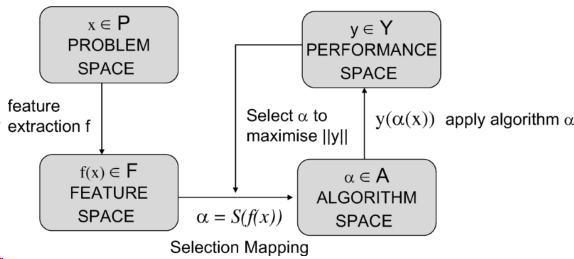
\includegraphics{./img/as_model.png}}
	\caption{Model of the AS problem}
	\label{fig:asmodel}
\end{figure}

An AS model is composed of four components: \textit{problems, features, algorithms,} and \textit{performance}.

\begin{enumerate}
	\item Problem space ($\mathbf{P}$) \\
	The set of problem instances. Instances are often grouped into \textit{problem classes}, which categorize their level of difficulty. The number of problems are usually vast and diverse.
	\item Feature space ($\mathbf{F}$) \\
	The set of features describing the problem instances. Specifically, features define the measurable characteristics of problems, which provides an indication on the difficulty of problems.
	\item Algorithm space ($\mathbf{A}$) \\
	The set of algorithms used to solving the problem instances. A large number of algorithms could be possibly used, but practically only a handful is considered.
	\item Performance space ($\mathbf{Y}$) \\
	The set of metrics that defines how algorithm performance is measured.
\end{enumerate}

Formally stating the AS problem, 

\fbox{
\begin{minipage}{\dimexpr\textwidth-1cm}
\textit{Given problem instance $x \in \mathbf{P}$ with features $f(x) \in \mathbf{F}$ , find a selection mapping $\alpha = S(f(x))$ in algorithm space $\mathbf{A}$, where the selected algorithm $\alpha \in \mathbf{A}$ provides the maximum performance $y(\alpha(x)) \in \mathbf{Y}$ in solving the problem instance $x \in \mathbf{P}$.}
\end{minipage}
}

\subsection{Motivation}
AS is based on the observation that there is no single algorithm that can optimally solve all kinds of problems. The \textit{No Free Lunch} (NFL) theorems assert that on a set of problems with varying degrees of difficulty, all algorithms perform the same on average \citep{wolpert1997no}. This implies that if an algorithm executes well on one class of problems, it pays off for decreased performance on other classes. NFL theorems have been demonstrated on problems such as search \citep{wolpert1995no}, cross validation \citep{goutte1997note}, multiobjective optimization \citep{corne2003no}, and sparse approximation \citep{xu2012sparse}.

\begin{figure}[H]
	\centering
	\scalebox{.6}{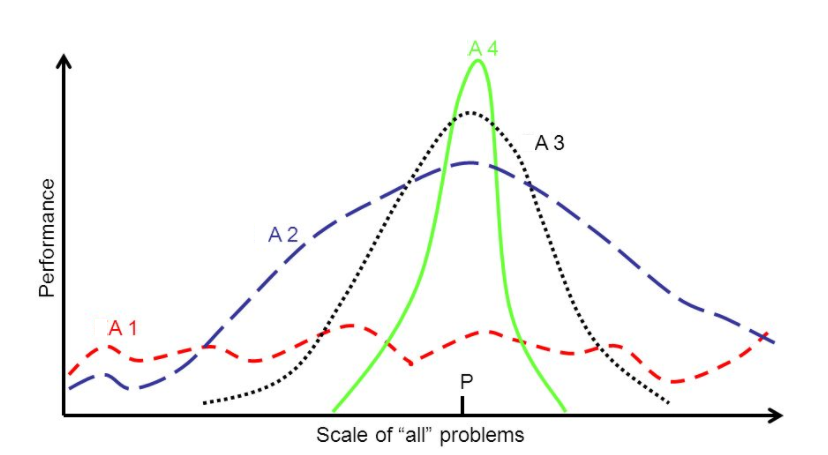
\includegraphics{./img/algo_perf_dist.png}}
	\caption{Typical distribution of algorithms with respect to performance}
	\label{fig:algoperfdist}
\end{figure}

The NFL theorems suggest to shift the focus of solving problems to AS. Learning the problem characteristics can help in deciding which algorithm is most suitable in solving a problem. Also, a set of algorithms with complementary strengths is desirable. A collection of algorithms used for solving a set of problems is called an \textit{algorithm portfolio}.

\subsection{Algorithm Portfolios}
Algorithm portfolios combine multiple algorithms with complementary strengths in order to solve problems more efficiently. This is inspired by \textit{investment portfolios} concept in Economics where maximizing a utility with associated risks is handled by mixing strategies with desired risk and performance \citep{huberman1997economics}.

\begin{figure}[H]      
	\scalebox{.7}{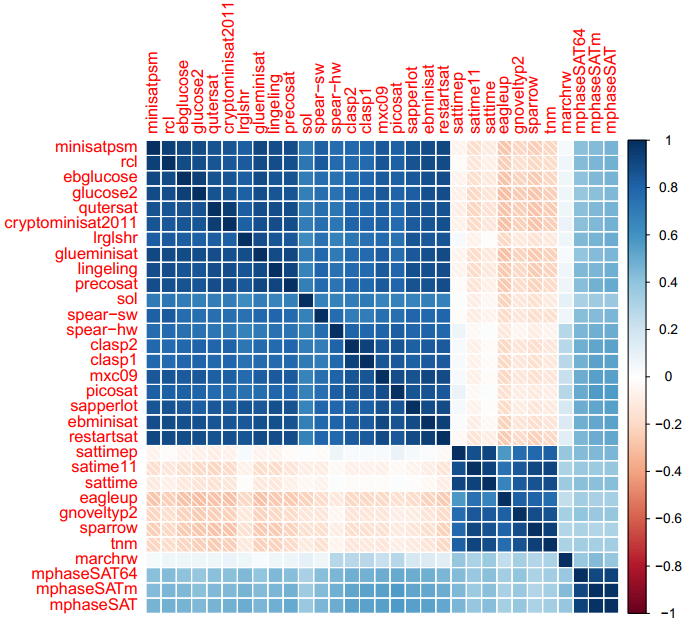
\includegraphics{./img/sat_correl.png}}
	\caption[Correlation matrix of SAT solvers]{Correlation matrix of SAT solvers. Solvers with less correlation have more complementary performance. Red and blue boxes indicate negative and positive correlation respectively; shading represents the correlation strength \citep{bischl2016aslib}}
	\label{fig:satcorrel}
\end{figure}

Using algorithm portfolios have been proven effective on solving hard combinatorial problems \citep{gomes2001algorithm}. Gomes and Selman concluded that algorithm portfolios can obtain superior performance by exploiting the variance in behavior among algorithms. One AS technique that takes advantage of this is called \textit{presolving}. Presolving makes use of \textit{presolvers}, which basically are algorithms that execute quickly and can solve a large number of problems \citep{xu2008satzilla}. Presolvers tend to eliminate the easier problems so AS can focus on solving the much harder problems.

\subsection{Problem Domain}
AS can be best applied on combinatorial search and optimization problems. One example is the Boolean satisfiability (SAT) problem, a classic NP-complete problem of finding assignments of variables to a Boolean formula such that it evaluates to TRUE. Successful AS implementations include SATzilla \citep{xu2008satzilla}, SATenstein \citep{khudabukhsh2009satenstein}, and Hydra \citep{xu2010hydra}. Efficient SAT solvers benefit applications such as IC design, computer-aided design and manufacturing, and automated theorem proving.

\begin{figure}[H]
	\centering
	\scalebox{.9}{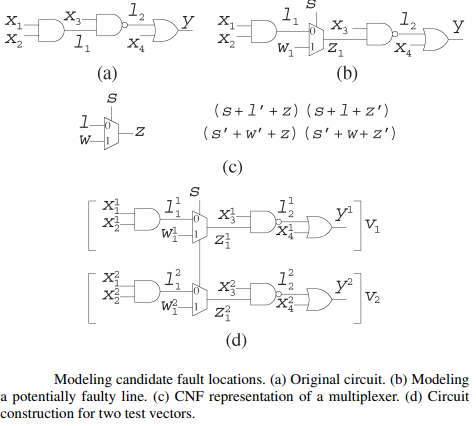
\includegraphics{./img/logic_circuits.png}}
	\caption[Fault-diagnosis of very-large-scale-integration (VLSI) circuits modelled as a SAT problem]{Fault-diagnosis of very-large-scale-integration (VLSI) circuits modelled as a SAT problem. \citep{smith2005fault}}
	\label{fig:logiccircuits}
\end{figure}

Travelling salesman problem (TSP), a famous example of an \textit{NP}-hard problem, also benefits from AS. Given a list of points and the associated costs between pairs of points, the goal of TSP is to find a path with minimum total cost between two selected points. Points can represent destinations or, in a more abstract sense, nodes in a graph. Costs can refer to distance or any measure that represents the weight of relationship between a pair of nodes in a graph. An algorithm portfolio of inexact TSP solvers showed significant performance improvements after AS \citep{kotthoff2015improving}. The travelling thief problem \citep{bonyadi2013travelling}, a combination of TSP and knapsack problem \citep{kellerer2004introduction}, has also been tackled using AS techniques, resulting in substantial improvements over single solvers \citep{wagner2018case}. 

\begin{figure}[H]
	\centering
	\scalebox{.6}{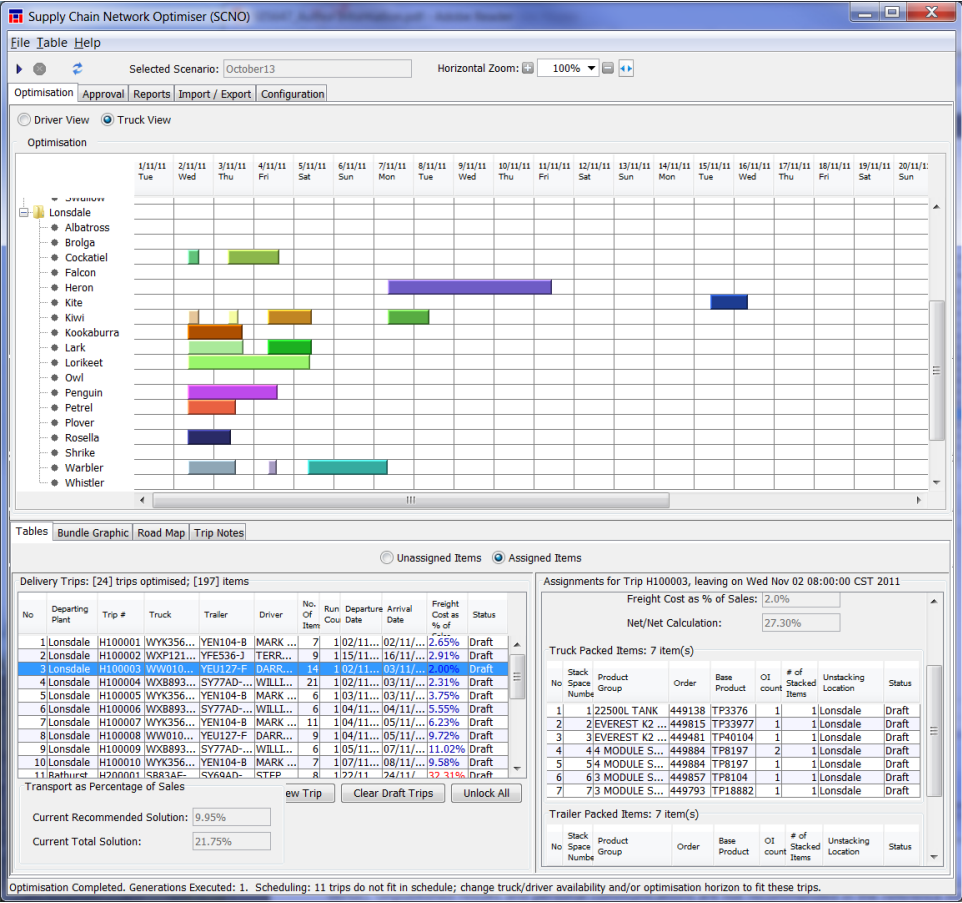
\includegraphics{./img/water_tank.png}}
	\caption[Water tank delivery schedule generated by an optimizer software]{Water tank delivery schedule generated by an optimizer software. This demonstrates the real-world application of the solution to travelling thief problem. \citep{stolk2013combining}}
	\label{fig:watertank}
\end{figure}

In this study, AS is applied on solving subgraph isomorphism problems. This is an \textit{NP}-complete problem whereby a smaller graph is located in a larger graph. As the number of graph nodes increases, the amount of effort expended in searching for subgraph isomorphisms exponentially increases. Using AS to search for subgraph isomorphisms have demonstrated significant performance improvements over standalone algorithms (\citet{battiti2007algorithm}; \citet{kotthoff2016portfolios}). Subgraph isomorphism problems manifest in applications that use graphs to model problems. A few examples include chemistry, software engineering, and biocomputing.

\begin{figure}[H]
	\centering
	\scalebox{.7}{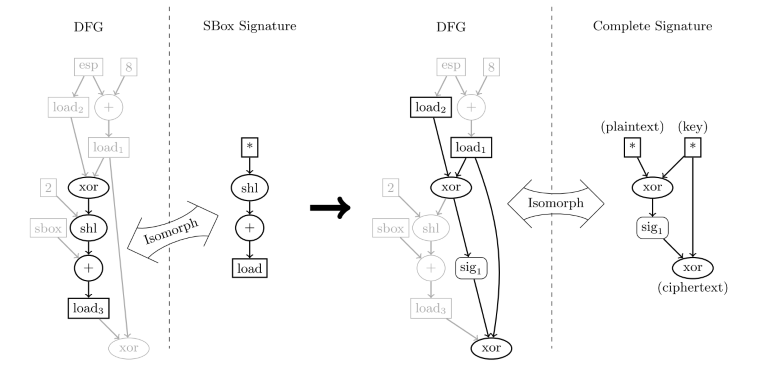
\includegraphics{./img/flowchart.png}}
	\caption[Identifying malware in executable files through recognition of cryptographic algorithm patterns]{Identifying malware in executable files through recognition of cryptographic algorithm patterns. Searching for a cryptographic signature (pattern graph) from the program's data flow graph (DFG) is a subgraph isomorphism problem. \citep{lestringant2015automated}}
	\label{fig:flowchart}
\end{figure}

Combining the strengths of several algorithms through AS can lead to more efficient solutions to hard combinatorial problems. In retrospect, AS does not entirely discourage the formulation of new algorithms. Research in AS seeks not only to improve problem solving performance, but also to learn more about the nature of problems and the behaviors of algorithms used. It can also provide valuable insights in creating new algorithms or improving upon existing ones. Studies on new algorithms are just as important as AS research, since the effectiveness of AS still relies on how well individual algorithms perform.

\section{Algorithm Selection Techniques}
A comprehensive review of AS techniques can be referred from Smith-Miles \citep{smith2009cross} and Kotthoff \citep{kotthoff2016algorithm}. Typically, the following are considered when creating a new AS technique:

\begin{enumerate}
	\item How can algorithm portfolios be constructed? (e.g. static portfolios vs. dynamic portfolios)
	\item What algorithms to select and when? (e.g. single algorithm per problem vs. multiple algorithms with scheduling)
	\item How to select algorithms? (modelling algorithm performance with respect to problems)
\end{enumerate}

This study is limited to the use of a static portfolio and the selection of one algorithm per problem instance. This section mainly discusses techniques in (3). 

On most approaches, machine learning is used to discover the relationship between algorithms and problems.  This often includes a training phase, where algorithms are executed on a subset of problems to evaluate their performance. The general approach to AS \citep{bischl2016aslib} is depicted in Figure \ref{fig:asworkflow}.

\begin{figure}[H]
	\centering
	\scalebox{.6}{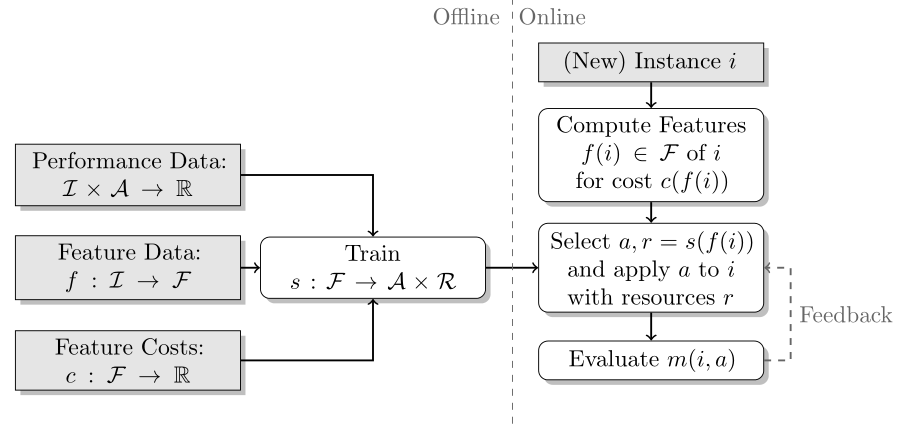
\includegraphics{./img/as_workflow.png}}
	\caption[AS workflow]{AS workflow.}
	\label{fig:asworkflow}
\end{figure}

\begin{enumerate}
	\item For each problem instance \textit{i}, a vector of instance features $f(i) \in \mathbf{F}$ is computed. 
	\item A machine learning technique \textit{s} selects an algorithm $a \in \mathbf{A}$ based on the feature vector from Step 1.
	\item The selected algorithm \textit{a} is applied to problem instance \textit{i}.
	\item Performance measure \textit{m} is evaluated, taking into account feature computation costs and the performance of the selected algorithm.
\end{enumerate}

Choosing a machine learning technique is often based from the nature of the problem to be solved. For instance, a classification model is viable for simple problem-algorithm mappings. Each problem can be labeled with the best-performing algorithm, then the classifier is trained to recognize problems and their corresponding optimal algorithms. One classifier implementation used a decision tree that assigned slower or faster algorithms to constraint satisfaction problems \citep{gent2010learning}. 

\begin{figure}[H]
	\centering
	\scalebox{.7}{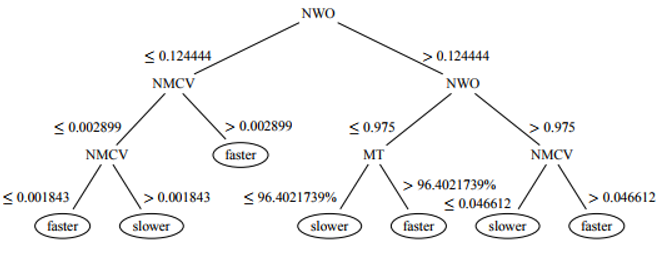
\includegraphics{./img/decision_tree.png}}
	\caption[Decision tree classifier built using C4.5 algorithm]{Decision tree classifier built using C4.5 algorithm.Nodes represent attribute rules the guide the decision of choosing a ‘slower’ or a ‘faster’ algorithm for a problem. \citep{gent2010learning}}
	\label{fig:decisiontree}
\end{figure}

Alternatively, algorithm performance can be predicted using regression models. Training is slower since it is done for each algorithm per problem instance, as opposed to classification models where training iterates only for each problem instance. The advantage is that models are learned per individual algorithm instead of the whole algorithm portfolio, as with the case for classification models. SATzilla, a SAT solver that dominated SAT competitions, used ridge regression to learn an AS model of SAT problems \citep{xu2008satzilla}. For subgraph isomorphism problems, pairwise random forest regression stands as the current best approach \citet{kotthoff2016portfolios}. 

\begin{figure}[H]
	\centering
	\scalebox{.7}{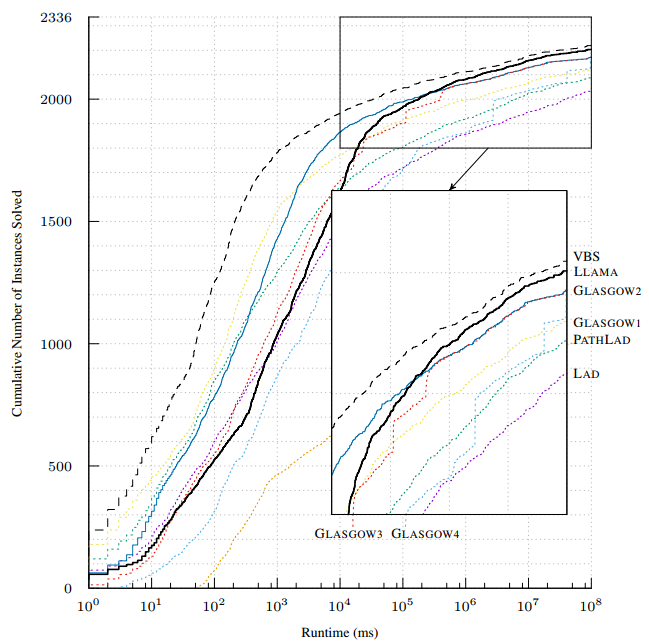
\includegraphics{./img/subgraph_isomorphism.png}}
	\caption[Performance comparison of subgraph isomorphism algorithms]{ Performance comparison of subgraph isomorphism algorithms. \textit{LLAMA} is the AS model trained using pairwise random forest regression. Its performance comes near the virtual best solver (VBS)—the upper-bound of what an AS model can achieve in an algorithm portfolio. \citep{kotthoff2016portfolios}}
	\label{fig:subgraphisomorphism}
\end{figure}

Another approach is to group problem instances into clusters and assign the cost-optimal solver for each cluster. This approach is useful when there is minimal knowledge about the problem. One example did not rely on problem features to do AS; instead a model of algorithm performance behavior is learned and then used to identify clusters of similar problems \citep{silverthorn2010latent}. The AS model gathered roughly competitive results after comparing against SATzilla.

\begin{table}[H]
	\centering
	\begin{tabular}{llll}
		\hline
		\multicolumn{1}{c}{\multirow{2}{*}{\textbf{Method}}} & \multicolumn{3}{c}{\textbf{SAT Instances Solved}} \\ \cline{2-4} 
		\multicolumn{1}{c}{} & \multicolumn{1}{c}{random} & \multicolumn{1}{c}{crafted} & \multicolumn{1}{c}{indust.} \\ \hline
		Best Single & 320.8 (3.7) & 122.6 (3.8) & \textbf{153.5 (3.2)} \\
		Random & 261.6 (4.8) & 89.3 (3.5) & 54.5 (3.4) \\
		SATzilla & 407.5 (3.1) & 125.6 (3.3) & 137.6 (3.3) \\
		Soft + Mult. & 319.3 (8.2) & 116.9 (4.9) & 136.2 (4.3) \\
		Soft + DCM & 342.2 (8.2) & 118.2 (4.3) & 138.1 (5.0) \\
		Hard + Mult. & 340.3 (45.7) & 104.8 (9.7) & 129.4 (8.0) \\
		Hard + DCM & \textbf{424.2 (12.9)} & \textbf{129.4 (6.5)} & 146.0 (5.6) \\ \hline
	\end{tabular}
	\caption[Comparison of the number of SAT problems solved between SATzilla vs. latent class clustering models]{Comparison of the number of SAT problems solved between SATzilla vs. latent class clustering models. The last four methods in the table correspond to different latent class methods used. \citep{silverthorn2010latent}}
	\label{tbl:satzilla}
\end{table}

Several machine-learning approaches to AS exist, such as hybrid regression-classification models \citep{kotthoff2012hybrid}, ensembles \citep{kotthoff2010ensemble}, and reinforcement learning \citep{lagoudakis2000algorithm}. 

\section{Reinforcement Learning Approach to Algorithm Selection}
Training AS models typically use classification or regression methods (or a hybrid of these two) due to the complete availability of information on problems and algorithm performance. Reinforcement learning (RL) techniques are typically used when dynamic (a.k.a. online learning) AS is necessary, where the AS model continuously adapts and learns as it solves more problems. One example is an AS model trained using a modified Q-learning algorithm \citep{lagoudakis2000algorithm}. The model continuously learns to select algorithms that minimize the overall time in solving all problems. A more sophisticated application used a multi-armed bandit approach to AS where the model progressively learns how to efficiently schedule and distribute problem solving across multiple CPUs \citep{gagliolo2009towards}.

RL encompasses computational methods in learning from interactions with the environment to achieve long term goals \citep{sutton1998reinforcement}. An \textit{agent} perceives the \textit{state} of its \textit{environment} and receives \textit{feedback} (instantly or time-delayed) for every \textit{action} it takes. Feedback can be understood as rewards in which the agent seek to maximize over time. Learning is driven by the interaction between agent and environment: the environment provides stimulus to the agent, and then the agent makes decisions on how to respond. In RL terms this is called \textit{policy} – a set of rules that guides agent behavior.

Figure \ref{fig:rlmodel} summarizes the main idea behind RL. The RL model can be framed in the context of AS by mapping its elements to the model of AS problem (Figure 2.1). This is shown in Figure \ref{fig:rlasmodel}.

\begin{figure}[H]
	\centering
	\scalebox{.5}{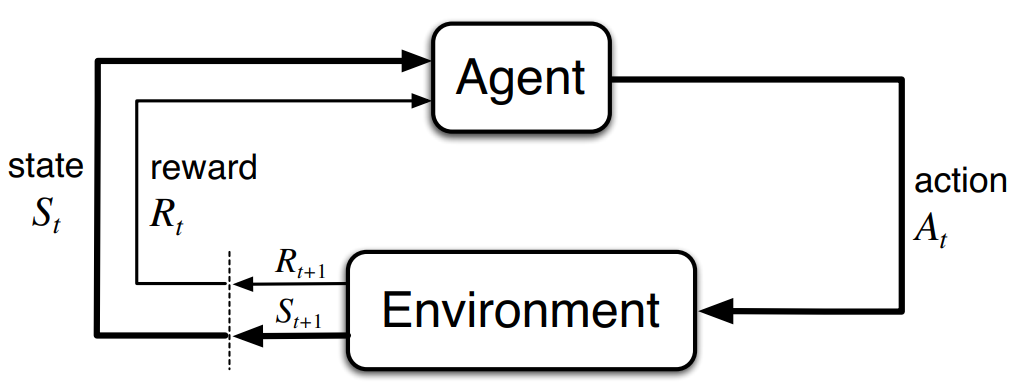
\includegraphics{./img/rl_model.png}}
	\caption{Reinforcement learning model}
	\label{fig:rlmodel}
\end{figure}

\begin{figure}[H]
	\centering
	\scalebox{.85}{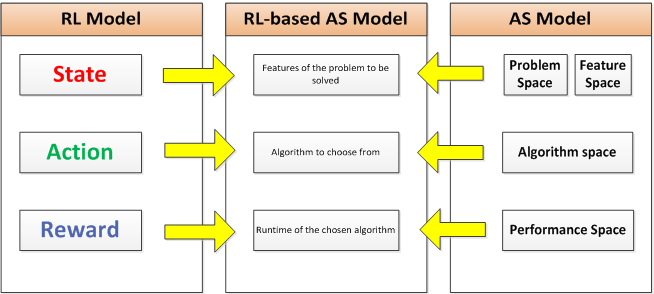
\includegraphics{./img/rlas_model.png}}
	\caption{Reinforcement learning-based algorithm selection model}
	\label{fig:rlasmodel}
\end{figure}

\subsection{Policy Gradient Methods}

The agent's \textit{policy} is a function that outputs an action based from the input environment state. It can be learned by applying some performance measure and monitoring how it changes with respect to the environment state. \textit{Policy gradient} methods represent a class of techniques under RL that learns a policy through change in performance measure. These methods seek to maximize long term rewards by optimizing performance.

\begin{equation}
\mathbf{\theta_{t+1}} = \mathbf{\theta_t} + \alpha \nabla J(\theta_t)
\label{eq:pgrad}
\end{equation}

This study uses REINFORCE algorithm \citep{williams1992simple} to train an AS model. The acronym describes the policy parameter update equation used in its algorithm: \textbf{RE}ward \textbf{IN}crement \textit{equals} \textbf{N}onnegative \textbf{F}actor \textit{plus} \textbf{O}ffset \textbf{R}einforcement \textit{plus} \textbf{C}haracteristic \textbf{E}ligibility. 

\begin{equation}
\mathbf{\theta_{t+1}} = \mathbf{\theta_t} + \alpha G_t \frac{\nabla_\theta\pi(A_t|S_t, \theta_t)}{\pi(A_t|S_t, \theta_t)}
\label{eq:reinforce}
\end{equation}

The intuition behind Equation \ref{eq:reinforce} is as follows: each increment is proportional to the product of a reward $G_t$ and a vector, the gradient of the probability of taking the action actually taken, $\nabla_\theta\pi(A_t|S_t, \theta_t)$, divided by the probability of taking that action $\pi(A_t|S_t, \theta_t)$. The vector is the direction in parameter space that most increases the probability of repeating the action $A_t$ on future visits to state $S_t$. The update increases the parameter vector in this direction proportional to the reward, and inversely proportional to the action probability. The former makes sense because it causes the parameter to move most in the directions that favor actions that yield the highest reward. The latter makes sense because otherwise actions that are selected frequently are at an advantage (the updates will be more often in their direction) and might win out even if they do not yield the highest return. \citep{sutton1998reinforcement}. 
\chapter{Research Methodology}
\section{Introduction}
This chapter discusses how the research is executed. An overview of the research methodology is provided in the research framework. The dataset and software used in conducting the experiments are explained in detail. The general approach on how AS models are constructed and evaluated is also discussed. 

\section{Research Framework}
\label{sec:researcframework}
The study underwent through four phases: \textit{Identify Research Problem}, \textit{Prepare Development Environment}, \textit{Build and Evaluate AS Model}, and \textit{Present Results}. The research flow is illustrated in Figure \ref{fig:researchframework}.

\begin{figure}[H]
	\centering
	\scalebox{.6}{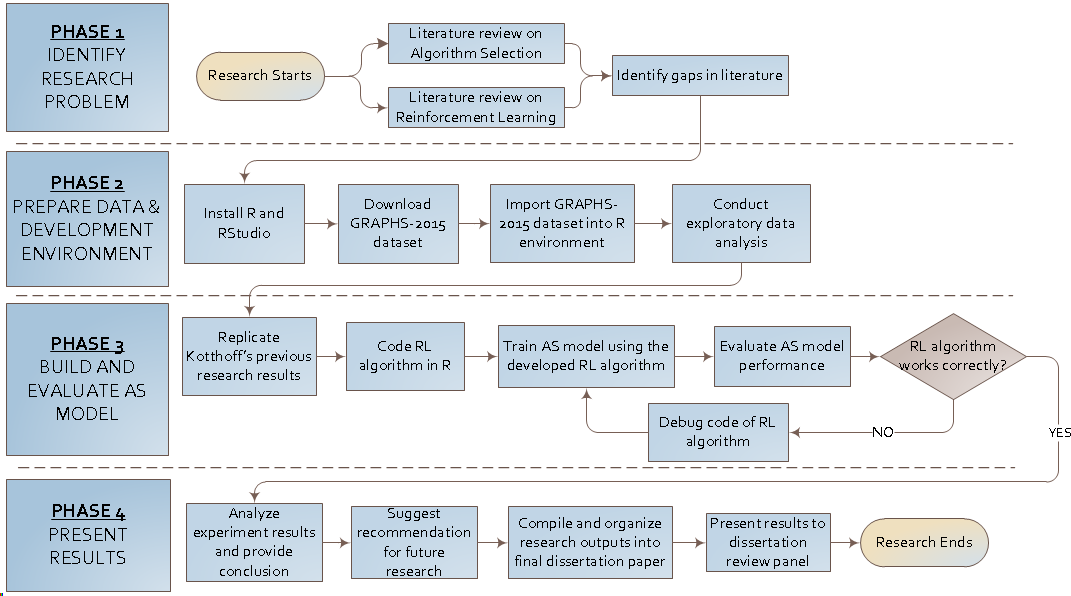
\includegraphics{./img/research_framework.png}}
	\caption{Research Framework} 
	\label{fig:researchframework}
\end{figure}

\section{Phase 1: Identify Research Problem} 
This research is inspired by the Open Algorithm Selection Challenge 2017 \citep{lindauer2017open} which showcased the latest techniques in AS. The datasets and tools used in the challenge have been made publicly available, allowing anyone to easily replicate the results. This lowers the barrier to entry to AS research.

The AS survey papers by Kotthoff \citep{kotthoff2016portfolios} and Smith-Miles \citep{smith2009cross} served as starting point in learning the background of AS. This study decided to focus on the application of AS to subgraph isomorphism problems. It has been chosen since a recent study of the same topic by Kotthoff and his colleagues \citep{kotthoff2016algorithm} published data and results that can be easily reproduced. This study is referred to a number of times in this paper and will henceforth abbreviated to PORTSUB for convenience. This study follows up on PORTSUB by proposing RL as an alternative in training AS models.

\section{Phase 2: Prepare Data and Development Environment} 
The experiments are executed on a server class desktop running Ubuntu Server 16.04 with 16 Gb RAM, Intel Xeon 4.0 GHz 12-core CPU, and an nVidia GeForce GTX1080Ti GPU. Experiments also ran well on a laptop installed with Windows 7 with 16 Gb RAM and Intel i7 3.0 GHz quad-core CPU. It is not really necessary to run the experiments on machines with specs as high as described since the computational requirements of training the AS models in this study are not very demanding. The experiments can be decently conducted on a Windows, MacOS, or GNU/Linux system with at least 4 Gb RAM and a 2.5 GHz quad-core CPU. 

\subsection{Install Development Software and Libraries}
All experiments are executed in R. R is a programming language for statistical computing and graphics. R’s capabilities suit well the experimental needs of this research, which include mostly data handling, data analysis, and plotting results. To develop in R, using an IDE such as RStudio is recommended. RStudio is an integrated set of tools that helps one to be more productive with R.

\begin{figure}[H]
	\centering
	\scalebox{.6}{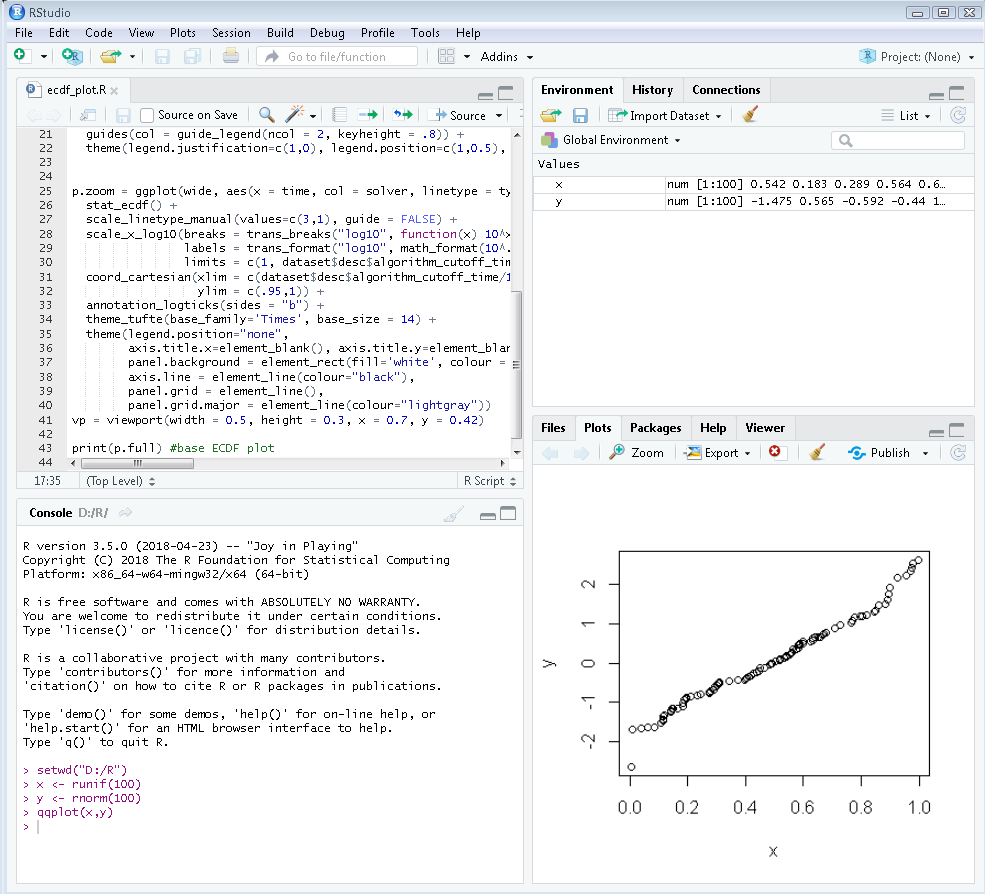
\includegraphics{./img/rstudio.png}}
	\caption{RStudio IDE} 
	\label{fig:rstudio}
\end{figure}

Libraries in R are called \textit{packages}. Packages bundle together code, data, documentation, and tests, and is easy to share with others \citep{wickham2015r}. Two R packages developed especially for AS research are available: these are ASlib and LLAMA.

\begin{figure}[H]
	\centering
	\scalebox{.8}{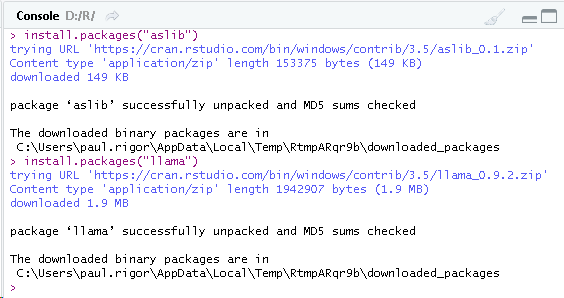
\includegraphics{./img/install_packages.png}}
	\caption{Installing packages in R} 
	\label{fig:installpackages}
\end{figure}

\subsubsection{Algorithm Selection Library (ASlib)}
Algorithm Selection Benchmark Library (ASlib) is an R package for operating on and analyzing AS datasets. This package allows researchers to work on AS problems and perform reproducible comparisons of approaches \citep{bischl2016aslib}. An ASlib dataset is called an \textit{AS scenario}. This contains pre-computed results for an algorithm portfolio on a set of problem instances, i.e., the performance measure is known for all pairs of algorithms and instances. In addition, the set of pre-computed instance features and its associated costs (the time spent in computing a feature) is provided for each instance. Providing this information makes it easy to build AS models, which typically involves (1) generating problem instances, (2) constructing an algorithm portfolio, (3) coding the algorithms, and (4) building the AS model. ASlib enables researchers to focus on (4) by providing the necessary data on (1) - (3). Furthermore, ASlib allows a fair and convenient evaluation and comparison of algorithm selectors.

The basic structure of an ASlib scenario is shown on \ref{tbl:aslibscenario}. The complete specification can be found online \citep{aslibspec}.

\begin{table}[H]
	\centering
	\begin{tabulary}{\textwidth}{|l|l|L|}
		\hline
		\multicolumn{1}{|c|}{\textbf{File Type}} & \multicolumn{1}{c|}{\textbf{Filename}} & \multicolumn{1}{c|}{\textbf{Description}} \\ \hline
		Meta information file & description.txt & Global description file containing general information about the scenario, including the name of the scenario, performance measures, algorithms, features and limitations of computational resources. \\ \hline
		Algorithm performance & algorithm\_runs.arff & Contains performance measurements with possible repetitions and completion status of the algorithm runs. The performance metric can be arbitrary, e.g., runtime, solution quality, accuracy or loss. \\ \hline
		Instance feature & feature\_values.arff & Contains the feature vectors for all instances. \\ \hline
		Feature costs & feature\_costs.arff & Contains the costs of the feature groups, i.e., sets of features computed together. \\ \hline
		Cross validation & cv.arff & Describes how to split the instance set into training and test sets to apply a standard machine learning approach to obtain an unbiased estimate of the performance of an algorithm selector. \\ \hline
	\end{tabulary}
	\caption{Basic structure of an ASlib scenario}
	\label{tbl:aslibscenario}
\end{table}


\subsubsection{Leveraging Learning to Automatically Manage Algorithms (LLAMA)}

Several previous studies implement AS models using different software environments like MATLAB and C++. Moreover, the implementations are highly tuned and customized for a particular problem domain. The Leveraging Learning to Automatically Manage Algorithms (LLAMA) R package addresses this problem by providing a common infrastructure for researchers to build, evaluate, and apply AS models \citep{kotthoff2013llama}. 

At a high level, LLAMA takes problem features and algorithm performance data as input (imported to R using ASlib package), feeds it to the AS model, and then outputs the model performance results. LLAMA contains built-in AS model training algorithms; it also allows custom ones to be implemented. Lastly, built-in performance measures in LLAMA include number of solved problems, misclassification penalty (MCP), and penalized average runtime (PAR) score.

\begin{figure}[H]
	\centering
	\scalebox{.8}{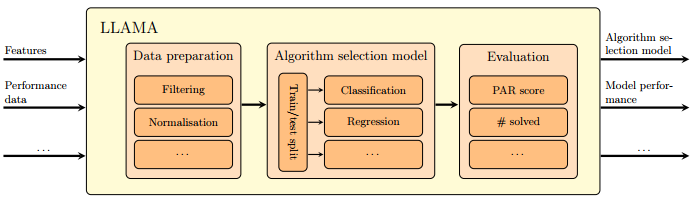
\includegraphics{./img/llama.png}}
	\caption{LLAMA framework}
	\label{fig:llama}
\end{figure}

\subsection{Prepare Dataset}
PORTSUB published a dataset called GRAPHS-2015, which is used to train and test the AS models in this study. It is available online in GitHub \citep{graphs2015} and is currently maintained by the Configuration and Selection of Algorithms (COSEAL) group.

\begin{figure}[H]
	\centering
	\scalebox{.6}{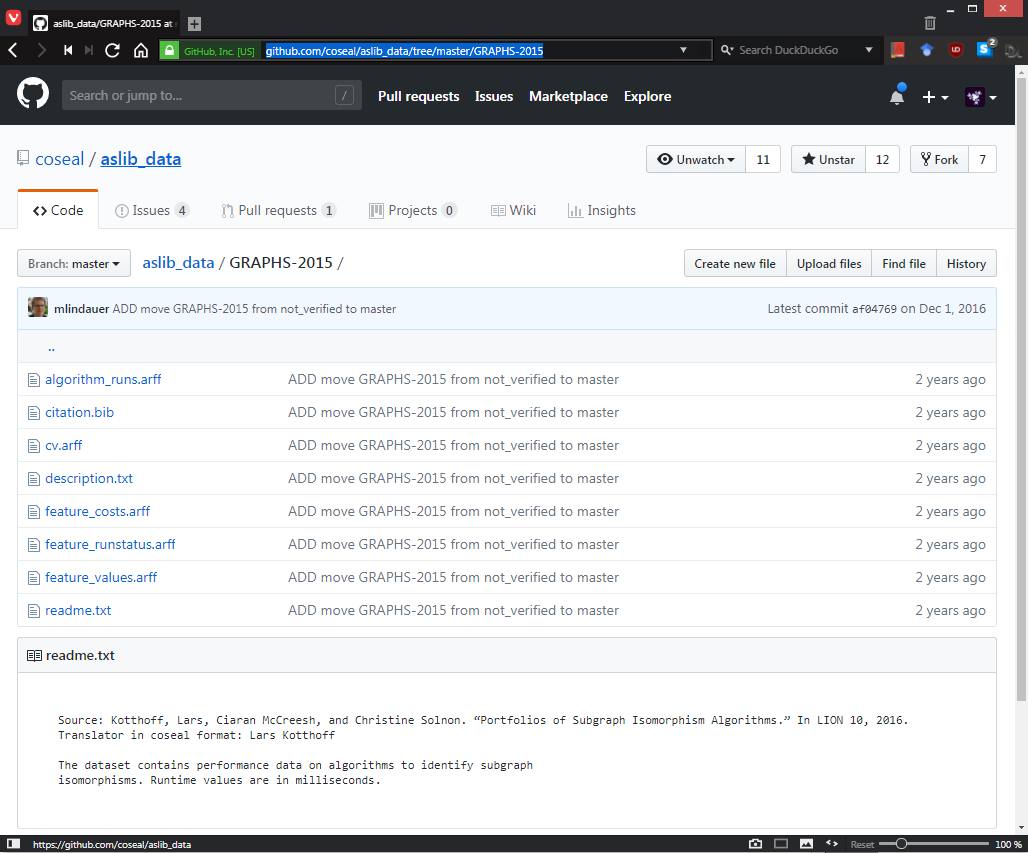
\includegraphics{./img/graphs2015github.png}}
	\caption[GRAPHS-2015 GitHub page]{GRAPHS-2015 GitHub page.}
	\label{fig:graphs2015github}
\end{figure}

\subsection{Replicate Previous Research Results}
The results of PORTSUB are replicated to verify its validity and to later serve as reference for benchmarking the AS model trained using RL. PORTSUB used a supervised learning technique called pairwise random forest regression (PRFR) to train an AS model in solving subgraph isomorphism problems. An implementation of this algorithm is readily available in LLAMA.

\section{Phase 3: Build and Evaluate AS Model}

An AS model is constructed in R, using the ASlib and LLAMA libraries to load the dataset and perform evaluation. The RL algorithm REINFORCE is studied and applied to AS of subgraph isomorphism problems. Its implementation utilized several functions found from the TensorFlow R package. TensorFlow is an open-source machine learning library used for high performance numerical computation \citep{abadi2016tensorflow}.

The effectiveness of AS is determined by comparing its performance against the virtual best solver (VBS) and the single best solver (SBS). VBS is the hypothetical model that does perfect AS, i.e., it always selects the best algorithm for each problem. SBS is the one algorithm from the algorithm portfolio that has the overall best performance across a set of problems. VBS defines the theoretical upper-bound performance that can be achieved by an AS model, while SBS defines the lower-bound performance. An AS model should at least get better performance than SBS to prove that AS is more effective than a single algorithm approach. An AS model becomes more effective as its performance gets closer to the VBS.

An AS model can be evaluated by its ability of how often it assigns the most optimal algorithms to a set of problems. In this study, the AS model performance is measured by calculating the mean misclassification penalty (MCP). This metric represents the additional time spent in solving problems when suboptimal algorithms were chosen. Individual algorithm performance is measured by its runtime, which is defined as the time taken by an algorithm to solve a problem instance. 

VBS, by its definition, always have mean MCP equal to zero. Lower MCP values signify better AS model performance. 


\begin{equation}
MCP = \frac{1}{N}\sum_{i=1}^{N}(t_{S_{i}} - t_{VBS_{i}})
\label{eq:mcp}
\end{equation}

where:

\begin{table}[H]
	\centering
	\begin{tabular}{rl}
		$N =$ & Total number of problem instances \\
		$t_{S_i} =$ & Runtime of the algorithm selected by the AS model \\
		$t_{VBS_i} =$ & Runtime of the algorithm selected by the VBS \\
		$i =$ & \textit{ith} problem instance
	\end{tabular}
\end{table}

\section{Phase 4: Present Results}

The last phase of this study compiles and organizes the findings into a full dissertation paper. The experiment results are discussed and conclusions are made. Lastly, recommendations for future research is presented.
\chapter{Algorithm Selection Model Training Algorithms}

\section{Introduction}
This chapter explains the implementation details of the algorithms used in training the AS model, which are \textit{pairwise random forest regression} (PRFR) and REINFORCE.

\section{Data Preparation}
\label{sec:dataprep}

Table \ref{tbl:graphs2015} displays the summary on GRAPHS-2015 dataset.

\begin{table}[H]
	\centering
	\begin{tabular}{|l|l|}
		\hline
		\textbf{Scenario ID} & GRAPHS-2015 \\ \hline
		\textbf{Source} & \citet{graphs2015} \\ \hline
		\textbf{Number of problem instances} & 5725 \\ \hline
		\textbf{Number of features} & 35 \\ \hline
		\textbf{Number of algorithms} & 7 \\ \hline
		\multirow{7}{*}{\textbf{Algorithm list}} & LAD \\ \cline{2-2} 
		& SupplementalLAD \\ \cline{2-2} 
		& VF2 \\ \cline{2-2} 
		& GLASGOW1 \\ \cline{2-2} 
		& GLASGOW2 \\ \cline{2-2} 
		& GLASGOW3 \\ \cline{2-2} 
		& GLASGOW4 \\ \hline
		\textbf{Performance measure} & Runtime (in milliseconds) \\ \hline
	\end{tabular}
	\caption{GRAPHS-2015 dataset summary}
	\label{tbl:graphs2015}
\end{table}

Only a subset of GRAPHS-2015 was used for training AS models. A technique called \textit{presolving} is used to eliminate the quickly solvable problem instances, leaving the harder problem instances for AS. The steps on removing presolved instances from GRAPHS-2015 were discussed in PORTSUB study. The flow and code is shown in Figures \ref{fig:presolver} and \ref{fig:extracthard}.

\begin{figure}[H]
	\centering
	\scalebox{.85}{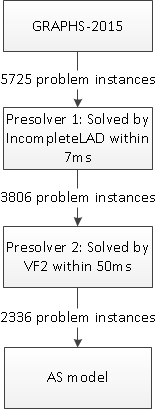
\includegraphics{./img/presolver.png}}
	\caption[Filtering presolved instances from GRAPHS-2015]{Filtering presolved instances from GRAPHS-2015. 2336 hard problems are left for AS.}
	\label{fig:presolver}
\end{figure}

\begin{figure}[H]
	\centering
	\scalebox{.60}{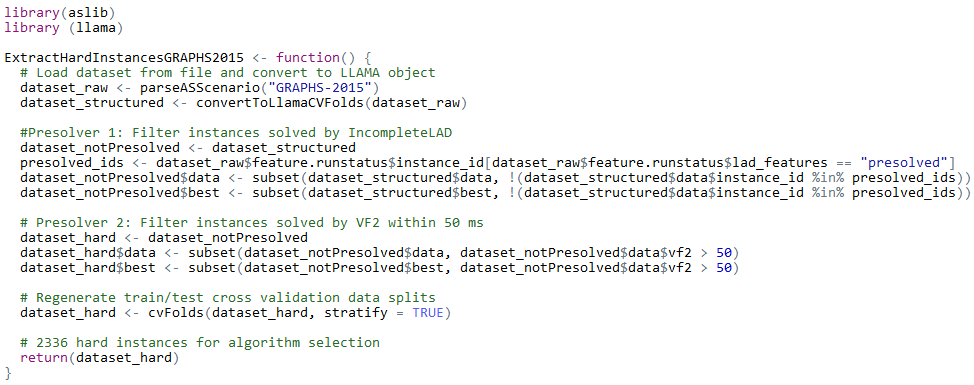
\includegraphics{./img/extract_hard_instances.png}}
	\caption{R script for extracting hard instances from GRAPHS-2015}
	\label{fig:extracthard}
\end{figure}

\section{Pairwise Random Forest Regression}
The AS model used in PORTSUB study was trained using a supervised learning approach called PRFR. It works as follows: for each pair of algorithms in the algorithm portfolio, a model is trained to predict the performance difference between them. If the first algorithm is better than the second, the difference is positive, otherwise negative. The algorithm with the highest cumulative performance difference, i.e. the most positive difference over all other algorithms, is chosen to be run. 

The LLAMA R package contains an implementation of pairwise random forest regression written by Lars Kotthoff, one of the PORTSUB authors. Its usage in R is shown on Figure \ref{fig:prfr}

\begin{figure}[H]
	\centering
	\scalebox{.65}{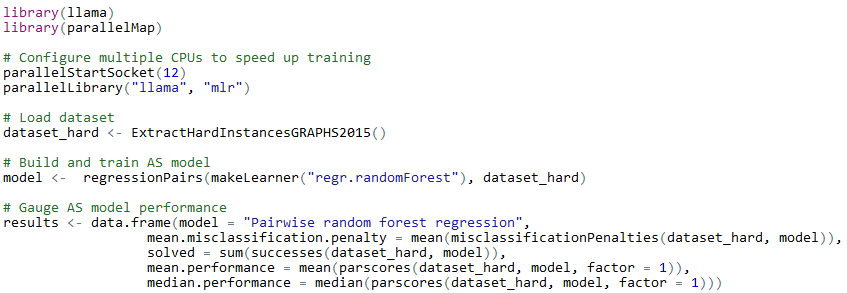
\includegraphics{./img/prfr.png}}
	\caption{R script for building AS model trained using PRFR}
	\label{fig:prfr}
\end{figure}

\section{REINFORCE}

The adaptation of REINFORCE algorithm to AS is composed of three main components:

\begin{enumerate}
	\item \textbf{Function approximator} \\
	An AS model can learn how algorithms match to problems with certain features. Patterns in problem features can be captured by function approximation methods, which translate feature values into parameters. For example, a simple function approximator such as linear regressor parameterizes inputs into slope and offset coefficients. Neural networks, a universal function approximator, represent parameters as network weights. Function approximation assists in generalizing AS model learning through discovery of feature patterns across problem instances.
	
	\item \textbf{Policy function} \\
	A policy function takes function approximator parameters as input and computes a probability for each algorithm. Algorithm probabilities change with respect to problem features. The computed probabilities serve as the basis of selection among algorithms.   
	
	\item \textbf{Reward function} \\
	The reward value is equivalent to the observed performance of the selected algorithm. It serves as feedback to the AS model to improve its capability in predicting optimal algorithms. Optionally, the reward value can be normalized or transformed to control how much the policy behavior should change with respect to feedback.  
\end{enumerate}

Figure \ref{fig:reinforce_flowchart} illustrates how an AS model is trained using \textit{REINFORCE} algorithm. 

\begin{figure}[H]
	\centering
	\scalebox{.65}{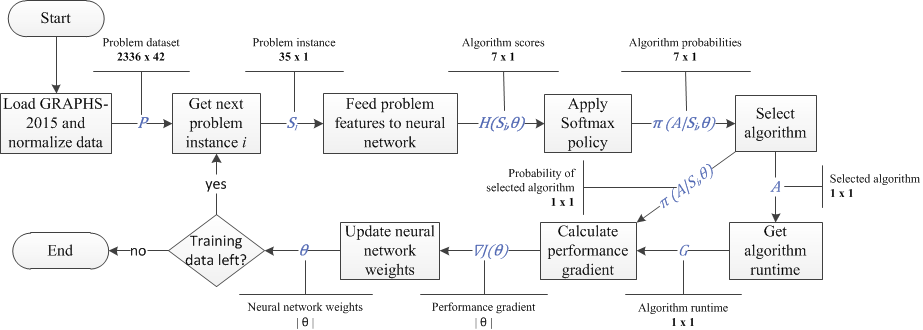
\includegraphics{./img/REINFORCE_flowchart.png}}
	\caption{Implementation of AS model trained using REINFORCE}
	\label{fig:reinforce_flowchart}
\end{figure}

\begin{enumerate}
	\item The GRAPHS-2015 dataset is loaded into R workspace. Hard problem instances are extracted, which consists of 2336 problem instances with 42 attributes used for training: 35 problem features plus runtime data of 7 algorithms.
	 
	\begin{figure}[H]
		\centering
		\scalebox{.75}{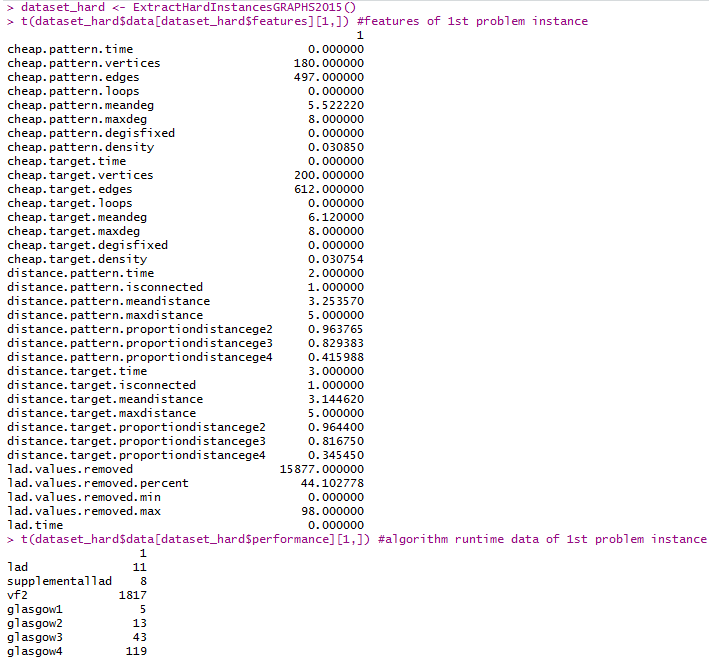
\includegraphics{./img/problem_instance.png}}
		\caption{Sample problem instance from GRAPHS-2015 dataset}
		\label{fig:problem_instance}
	\end{figure}

	\item Problem features are normalized using \textit{Z-score}. Normalization standardizes the range of data inputs which helps in resolving numerical issues when gradients are calculated during backpropagation. In effect, this speeds up neural network learning.
	
	\begin{equation}
	z_{ij} = \frac{x_{ij} - \mu_j}{\sigma_j}
	\end{equation} 
	
	where:
	
	\begin{table}[H]
		\centering
		\begin{tabular}{rl}
			$z_{ij} =$ & normalized feature value\\
			$x_{ij} =$ & feature value \\
			$\mu_{j} =$ & mean of \textit{jth} feature across \textbf{P} problem instances \\
			$\sigma_j =$ & standard deviation of \textit{jth} feature across \textbf{P} problem instances \\
			$\mathit{i} =$ & \textit{ith} instance from \textbf{P} problem instances \\
			$\mathit{j} =$ & \textit{jth} feature out of 35 features \\			
		\end{tabular}
	\end{table}

	The algorithm runtime data is rescaled to simplify the reward value used for computing the performance gradient. This enables the AS model to learn the most important information during problem solving, which is the ranking of algorithm performance from best to worst. This information is more important than the knowledge of actual algorithm runtimes, as the objective of AS is mainly not to characterize individual algorithm performance, but to determine which algorithms work best on problems. Table \ref{tbl:rewardscaling} shows how this study mapped algorithm ranking (determined by sorting runtime from shortest to longest) to reward values.

	\begin{table}[H]
		\centering
		\begin{tabular}{|c|c|}
			\hline
			\multicolumn{1}{|l|}{\textbf{Algorithm rank}} & \multicolumn{1}{l|}{\textbf{Assigned Reward Value}} \\ \hline
			1 & 16 \\ \hline
			2 & 4 \\ \hline
			3 & 1 \\ \hline
			4 & -4 \\ \hline
			5 & -16 \\ \hline
			6 & -64 \\ \hline
			7 & -256 \\ \hline
		\end{tabular}
		\caption{Algorithm ranking reward values}
		\label{tbl:rewardscaling}
	\end{table}
	
	\item A neural network is trained to map problem features (input) to algorithm scores (output). It is composed of an input layer with 35 inputs, 3 hidden layers, and an output layer with 7 outputs. Algorithm scores represent selection preferences, i.e., the larger the score, the more often that algorithm is taken.
	
	\item The algorithm scores are converted into probabilities using the softmax policy function. The probability assigned to an algorithm is proportional to its score, i.e., algorithms with the highest scores are given the highest probabilities of being selected. The softmax equation is given in the Equation below:
	
	\begin{equation}
	\pi(A | S_i, \theta) = \frac{\exp{H_A(S_i, \theta)}}{\sum_{b=1}^{7}\exp{H_b(S_i, \theta)}}
	\end{equation}
	
	where:
	
	\begin{table}[H]
		\centering
		\begin{tabular}{rl}
			$\pi(A | S_i, \theta) =$ & Probability of algorithm A \\
			$H_A(S_i, \theta) =$ & Algorithm score of algorithm A \\
			$H_B(S_i, \theta) =$ & Algorithm score of algorithm B \\
			$S_i =$ & features of problem instance \textit{i} \\
			$\theta =$ & neural network weights
		\end{tabular}
	\end{table}

	\item An algorithm is randomly selected based from the probabilities generated from the softmax policy function.
	
	\item The rescaled reward value corresponding to the selected algorithm is read from the dataset. This value, along with the probability of the selected algorithm, is used to calculate the performance gradient:
	
	\begin{equation}
	\nabla J(\theta_t) = G_t\ln{\pi(A | S_i, \theta_t)}
	\end{equation}
	
	where:
	
	\begin{table}[H]
		\centering
		\begin{tabular}{rl}
			$\nabla J(\theta_t) =$ & performance gradient \\
			$G_t =$ & reward \\
			$\pi(A | S_i, \theta_t) =$ & Probability of selected algorithm
		\end{tabular}
	\end{table}

	\item The performance gradient is used for backpropagation, a standard method of updating the weights of a neural network. Through this process, the neural network learns to adjust the algorithm scores in proportion to the reward value associated with the selected algorithm. 
	
	\begin{equation}
	\theta_{t+1} \gets \theta_t + \alpha \nabla J(\theta_t)
	\end{equation}
	
	where:
	
	\begin{table}[H]
		\centering
		\begin{tabular}{rl}
			$\theta_{t+1} =$ & Updated neural network weights \\
			$\theta_t =$ & current neural network weights \\
			$\alpha =$ & learning rate \\
			$\nabla J(\theta_t) =$ & performance gradient
		\end{tabular}
	\end{table}
\end{enumerate}

\section{Model Evaluation}
The performance of PRFR and REINFORCE are evaluated using 10-fold cross validation. The 2336 hard instances from GRAPHS-2015 are randomly partitioned into 10 subsets of approximately equal size. Of the 10 subsets, 9 are combined to form the training set for the AS models, while the remaining subset is formed as a test set. Mean MCP (Equation \ref{eq:mcp}) is calculated on the test set to evaluate the AS model performance. This is repeated 10 times for all possible combinations of training and test sets. At the end of this process, the final mean MCP is calculated by averaging the mean MCPs from all test sets.

\section{R source code implementation}
The implementation of AS models in this study can be retrieved from here: \url{https://github.com/kvrigor/algosel-rl}
\chapter{Experiment Results}

\section{Introduction}
This chapter presents the results from performing the experiments. The characteristics of the dataset are summarized on the exploratory data analysis section. The last section compares PRFR and REINFORCE in terms of their effectiveness in training an AS model for solving subgraph isomorphism problems.

\section{Exploratory Data Analysis}
\subsection{Data Summary}

The following statistical measures were taken for the results of each feature and algorithm:

\begin{itemize}
	\item \textbf{min} - minimum
	\item \textbf{qu\_-1st} - 25\% quantile
	\item \textbf{med} - median
	\item \textbf{mean} -  arithmetic mean
	\item \textbf{qu\_3rd} - 75\%-quantile
	\item \textbf{max} - maximum
	\item \textbf{sd} - standard deviation
	\item \textbf{coeff\_var} - coefficient of variation (standard deviation / arithmetic mean)
\end{itemize}

\begin{table}[H]
	\centering
	\resizebox{\columnwidth}{!}{%
	\begin{tabular}{|l|r|r|r|r|r|r|r|r|}
		\hline
		\multicolumn{1}{|c|}{\textbf{Features}} & \multicolumn{1}{c|}{\textbf{min}} & \multicolumn{1}{c|}{\textbf{qu\_1st}} & \multicolumn{1}{c|}{\textbf{med}} & \multicolumn{1}{c|}{\textbf{mean}} & \multicolumn{1}{c|}{\textbf{qu\_3rd}} & \multicolumn{1}{c|}{\textbf{max}} & \multicolumn{1}{c|}{\textbf{sd}} & \multicolumn{1}{c|}{\textbf{coeff\_var}} \\ \hline
		cheap.pattern.time                      & 0.0000                            & 0.0000                                & 0.0000                            & 0.0035                             & 0.0000                                & 1.0000                            & 0.0590                           & 16.8908                                  \\ \hline
		cheap.pattern.vertices                  & 4.0000                            & 48.0000                               & 80.0000                           & 109.3787                           & 128.0000                              & 900.0000                          & 114.9942                         & 1.0513                                   \\ \hline
		cheap.pattern.edges                     & 4.0000                            & 112.0000                              & 240.0000                          & 598.8704                           & 696.0000                              & 12410.0000                        & 1073.5139                        & 1.7926                                   \\ \hline
		cheap.pattern.loops                     & 0.0000                            & 0.0000                                & 0.0000                            & 0.2451                             & 0.0000                                & 9.0000                            & 1.3121                           & 5.3543                                   \\ \hline
		cheap.pattern.meandeg                   & 1.7867                            & 3.6364                                & 5.4286                            & 10.4274                            & 10.0000                               & 99.0000                           & 14.4378                          & 1.3846                                   \\ \hline
		cheap.pattern.maxdeg                    & 2.0000                            & 8.0000                                & 11.0000                           & 20.6091                            & 26.0000                               & 269.0000                          & 27.3313                          & 1.3262                                   \\ \hline
		cheap.pattern.degisfixed                & 0.0000                            & 0.0000                                & 0.0000                            & 0.1132                             & 0.0000                                & 1.0000                            & 0.3168                           & 2.7993                                   \\ \hline
		cheap.pattern.density                   & 0.0045                            & 0.0441                                & 0.0978                            & 0.1683                             & 0.1830                                & 1.0000                            & 0.2194                           & 1.3038                                   \\ \hline
		cheap.target.time                       & 0.0000                            & 0.0000                                & 0.0000                            & 3.9988                             & 2.0000                                & 55.0000                           & 9.5821                           & 2.3963                                   \\ \hline
		cheap.target.vertices                   & 10.0000                           & 216.0000                              & 561.0000                          & 1147.3385                          & 1430.0000                             & 6671.0000                         & 1440.1846                        & 1.2552                                   \\ \hline
		cheap.target.edges                      & 15.0000                           & 930.0000                              & 2074.0000                         & 7176.6114                          & 5994.0000                             & 209000.0000                       & 21594.1676                       & 3.0090                                   \\ \hline
		cheap.target.loops                      & 0.0000                            & 0.0000                                & 0.0000                            & 1.6306                             & 0.0000                                & 144.0000                          & 13.3146                          & 8.1656                                   \\ \hline
		cheap.target.meandeg                    & 0.4357                            & 4.1983                                & 6.0000                            & 19.4312                            & 11.9172                               & 270.6950                          & 39.8146                          & 2.0490                                   \\ \hline
		cheap.target.maxdeg                     & 2.0000                            & 10.0000                               & 19.0000                           & 102.2134                           & 52.0000                               & 4973.0000                         & 384.0174                         & 3.7570                                   \\ \hline
		cheap.target.degisfixed                 & 0.0000                            & 0.0000                                & 0.0000                            & 0.1492                             & 0.0000                                & 1.0000                            & 0.3563                           & 2.3885                                   \\ \hline
		cheap.target.density                    & 0.0005                            & 0.0030                                & 0.0119                            & 0.0729                             & 0.0588                                & 1.0000                            & 0.1585                           & 2.1736                                   \\ \hline
		distance.pattern.time                   & 0.0000                            & 0.0000                                & 0.0000                            & 2.0349                             & 1.0000                                & 93.0000                           & 8.0467                           & 3.9543                                   \\ \hline
		distance.pattern.isconnected            & 0.0000                            & 1.0000                                & 1.0000                            & 0.7976                             & 1.0000                                & 1.0000                            & 0.4019                           & 0.5039                                   \\ \hline
		distance.pattern.meandistance           & 1.0000                            & 2.0010                                & 2.7778                            & 3.9349                             & 4.1227                                & 80.6687                           & 5.6418                           & 1.4338                                   \\ \hline
		distance.pattern.maxdistance            & 1.0000                            & 3.0000                                & 5.0000                            & 8.9328                             & 9.0000                                & 240.0000                          & 16.9947                          & 1.9025                                   \\ \hline
		distance.pattern.proportiondistancege2  & 0.0000                            & 0.6000                                & 0.8466                            & 0.7406                             & 0.9319                                & 0.9929                            & 0.2661                           & 0.3593                                   \\ \hline
		distance.pattern.proportiondistancege3  & 0.0000                            & 0.0974                                & 0.5000                            & 0.4605                             & 0.8237                                & 0.9834                            & 0.3507                           & 0.7615                                   \\ \hline
		distance.pattern.proportiondistancege4  & 0.0000                            & 0.0000                                & 0.1957                            & 0.3091                             & 0.6094                                & 0.9752                            & 0.3225                           & 1.0432                                   \\ \hline
		distance.target.time                    & 0.0000                            & 5.0000                                & 32.0000                           & 553.0529                           & 208.0000                              & 9962.0000                         & 1474.8373                        & 2.6667                                   \\ \hline
		distance.target.isconnected             & 0.0000                            & 0.0000                                & 1.0000                            & 0.7095                             & 1.0000                                & 1.0000                            & 0.4540                           & 0.6399                                   \\ \hline
		distance.target.meandistance            & 1.0000                            & 2.4484                                & 3.7010                            & 7.4919                             & 7.1508                                & 100.6250                          & 11.7237                          & 1.5648                                   \\ \hline
		distance.target.maxdistance             & 1.0000                            & 5.0000                                & 8.0000                            & 16.3768                            & 16.0000                               & 200.0000                          & 24.8081                          & 1.5148                                   \\ \hline
		distance.target.proportiondistancege2   & 0.0000                            & 0.6082                                & 0.9502                            & 0.7944                             & 0.9900                                & 0.9993                            & 0.2896                           & 0.3645                                   \\ \hline
		distance.target.proportiondistancege3   & 0.0000                            & 0.2472                                & 0.7260                            & 0.5990                             & 0.9502                                & 0.9985                            & 0.3708                           & 0.6190                                   \\ \hline
		distance.target.proportiondistancege4   & 0.0000                            & 0.0288                                & 0.3875                            & 0.4514                             & 0.8813                                & 0.9973                            & 0.3838                           & 0.8502                                   \\ \hline
		lad.values.removed                      & 0.0000                            & 0.0000                                & 0.0000                            & 28733.8725                         & 10673.0000                            & 844304.0000                       & 81827.2598                       & 2.8478                                   \\ \hline
		lad.values.removed.percent              & 0.0000                            & 2.3503                                & 49.2371                           & 51.7472                            & 100.0000                              & 100.0000                          & 41.8261                          & 0.8083                                   \\ \hline
		lad.values.removed.min                  & 0.0000                            & 0.0000                                & 0.0000                            & 6.7000                             & 0.3190                                & 99.9700                           & 19.4023                          & 2.8959                                   \\ \hline
		lad.values.removed.max                  & 0.0000                            & 0.0000                                & 0.0000                            & 33.1602                            & 88.2143                               & 99.9816                           & 42.8695                          & 1.2928                                   \\ \hline
		lad.time                                & 0.0000                            & 0.0000                                & 0.0000                            & 7.1210                             & 3.0000                                & 3964.0000                         & 80.7295                          & 11.3367                                  \\ \hline
	\end{tabular}%
}
\caption{Summary of features}
\label{tbl:featuresummary}
\end{table}

\begin{table}[H]
	\centering
	\resizebox{\columnwidth}{!}{%
		\begin{tabular}{|l|r|r|r|r|r|r|r|r|}
			\hline
			\multicolumn{1}{|c|}{\textbf{Algorithm}} & \multicolumn{1}{c|}{\textbf{min}} & \multicolumn{1}{c|}{\textbf{qu\_1st}} & \multicolumn{1}{c|}{\textbf{med}} & \multicolumn{1}{c|}{\textbf{mean}} & \multicolumn{1}{c|}{\textbf{qu\_3rd}} & \multicolumn{1}{c|}{\textbf{max}} & \multicolumn{1}{c|}{\textbf{sd}} & \multicolumn{1}{c|}{\textbf{coeff\_var}} \\ \hline
			lad                                      & 0                                 & 3                                     & 33                                & 5935035.15                         & 1214                                  & 1.00E+08                          & 22874350.97                      & 3.8541                                   \\ \hline
			supplementallad                          & 0                                 & 3                                     & 22                                & 4841120.76                         & 402                                   & 1.00E+08                          & 20810140.52                      & 4.2986                                   \\ \hline
			vf2                                      & 0                                 & 6                                     & 115                               & 27565110.75                        & 1.00E+08                              & 1.00E+08                          & 44243664.13                      & 1.6051                                   \\ \hline
			glasgow1                                 & 0                                 & 4                                     & 25                                & 4158094.27                         & 199                                   & 1.00E+08                          & 19437830.22                      & 4.6747                                   \\ \hline
			glasgow2                                 & 0                                 & 12                                    & 61                                & 3196878.81                         & 414                                   & 1.00E+08                          & 17126177.54                      & 5.3572                                   \\ \hline
			glasgow3                                 & 0                                 & 33                                    & 168                               & 3212027.69                         & 1072                                  & 1.00E+08                          & 17153623.91                      & 5.3404                                   \\ \hline
			glasgow4                                 & 0                                 & 113                                   & 478                               & 4333647.25                         & 7178                                  & 1.00E+08                          & 19233485.20                      & 4.4382                                   \\ \hline
		\end{tabular}%
	}
	\caption[Summary of algorithms]{Summary of algorithms. All values represent runtime in milliseconds.}
	\label{tbl:algosummary}
\end{table}

\subsection{Distributions}
Histograms for features and algorithm runtimes are displayed in the following plots. The red dashed lines denote the median of the distribution.

\begin{figure}[H]
	\centering
	\scalebox{.65}{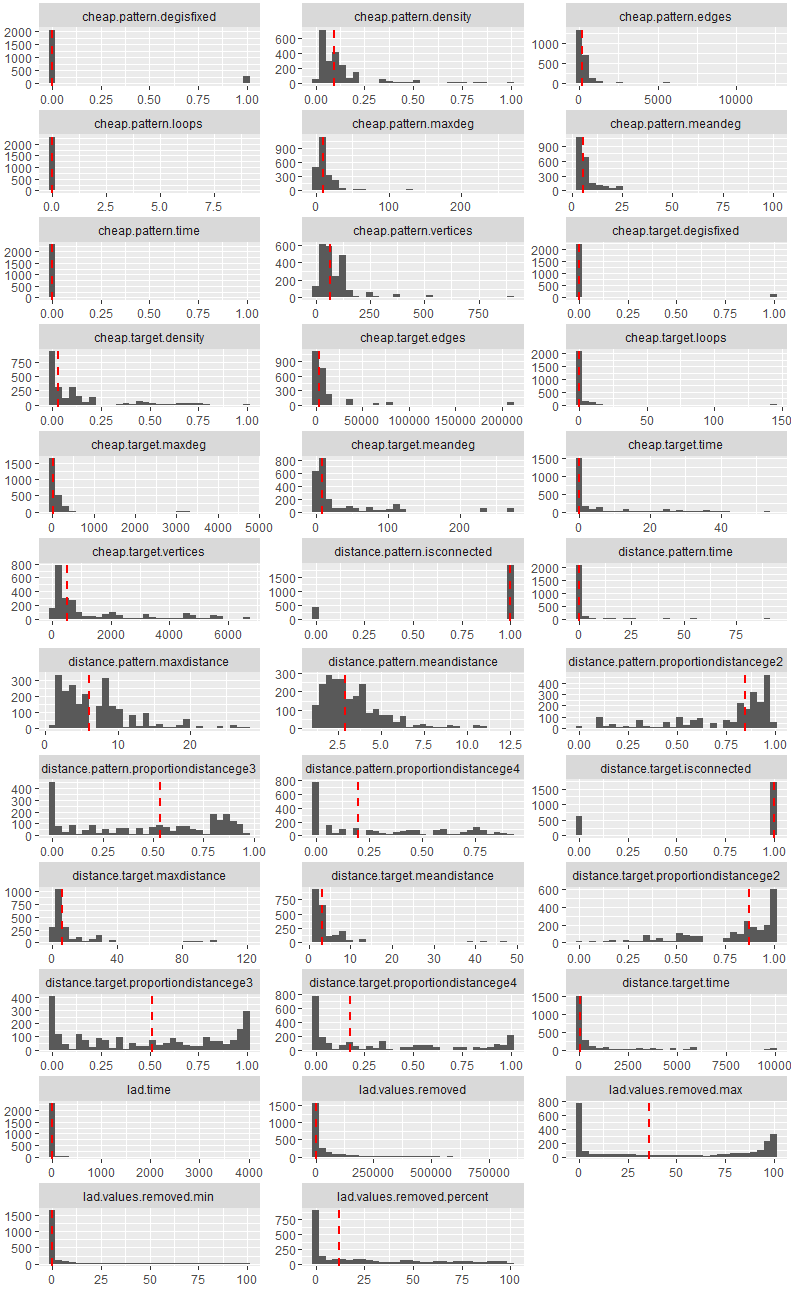
\includegraphics{./img/featuredist.png}}
	\caption{Feature distributions}
	\label{fig:featuredist}
\end{figure}

\begin{figure}[H]
	\centering
	\scalebox{.55}{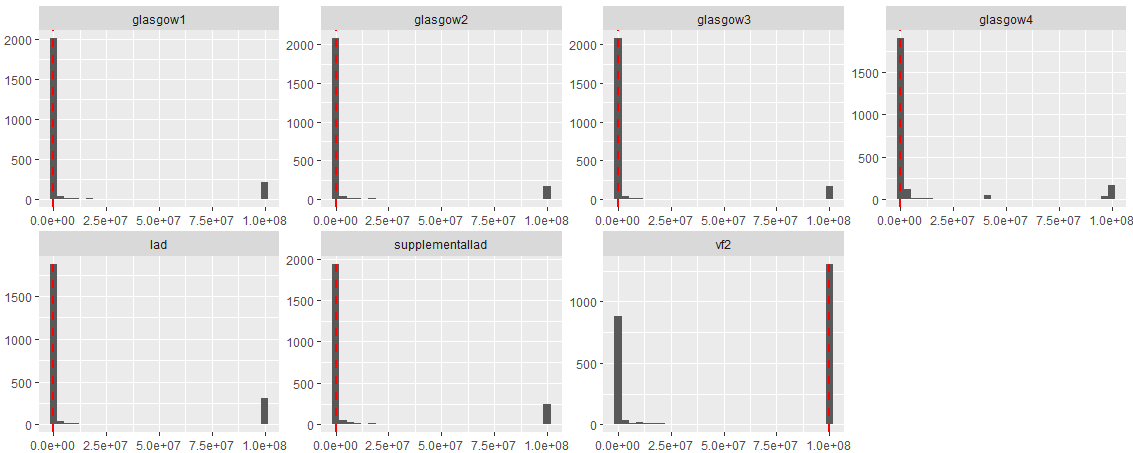
\includegraphics{./img/algodist.png}}
	\caption{Algorithm distributions}
	\label{fig:algodist}
\end{figure}

\begin{figure}[H]
	\centering
	\scalebox{.55}{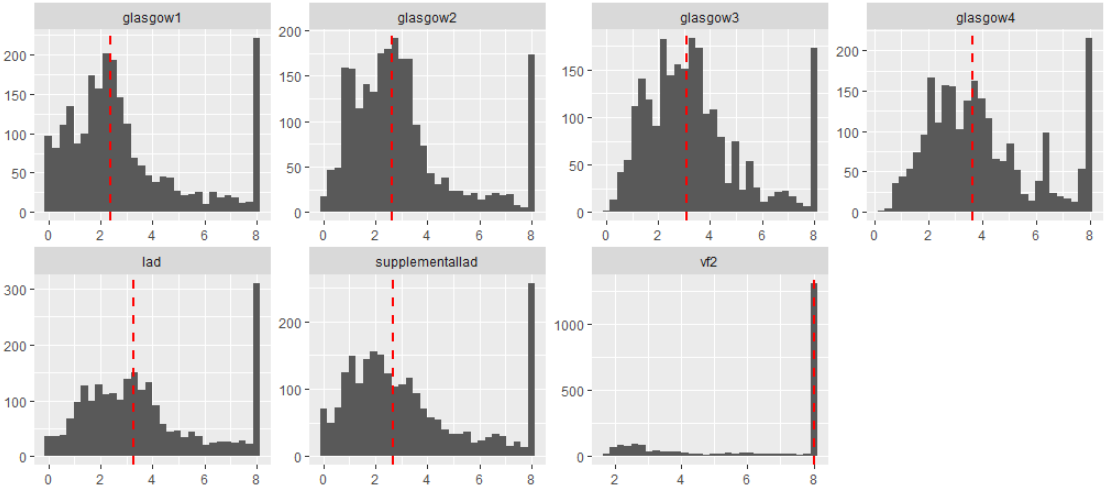
\includegraphics{./img/logalgodist.png}}
	\caption{Log-scaled algorithm distributions}
	\label{fig:logalgodist}
\end{figure}

\section{AS Model Performance Evaluation}

The mean MCP of the AS model trained using REINFORCE is 4x worse than one trained using PRFR. REINFORCE is not able to surpass the performance standard set by PORTSUB, which was hoped to be surpassed in this study.

\begin{table}[H]
	\begin{tabular}{|l|l|l|l|l|}
		\hline
		\textbf{AS Model} & \textbf{Mean MCP} & \textbf{\# Solved problems} & \textbf{Mean Performance} & \textbf{Median Performance} \\ \hline
		VBS               & 0.0               & 2,219                       & 5,822,809.0               & 79.0                        \\ \hline
		PRFR              & 621,662.5         & 2,208                       & 6,446,129.0               & 1,748.5                     \\ \hline
		SBS               & 1,963,498.6       & 2,173                       & 7,786,308.0               & 539.0                       \\ \hline
		REINFORCE         & 2,318,832.0       & 2,156                       & 8,168,306.0               & 929.0                       \\ \hline
	\end{tabular}
	\caption{AS model performance evaluation results}
	\label{tbl:asresults}
\end{table}

Despite REINFORCE failing to obtain better MCP than PRFR, it showed improvement on median performance, reporting almost 2x better than PRFR.  Its significance becomes clearer by analyzing the cumulative density function (CDF) plot which visualizes the distribution of runtimes of the selected algorithms on all problems, as illustrated Figure \ref{fig:cdf}.  REINFORCE is able to select more optimal algorithms than PRFR on the easier problems (solvable within $10-10^4$ ms) on the dataset. For difficult problems which are solvable within at least 105-108 ms, REINFORCE selected worse-performing algorithms than PRFR. Although the easier problems constitute the majority (75\%) of the dataset, its influence on the mean MCP is much lesser than the harder problems. REINFORCE performed better than PRFR in solving the easy problems, but underperformed when it came to solving the more difficult problems. 

\begin{figure}[H]	
	\centering
	\scalebox{.9}{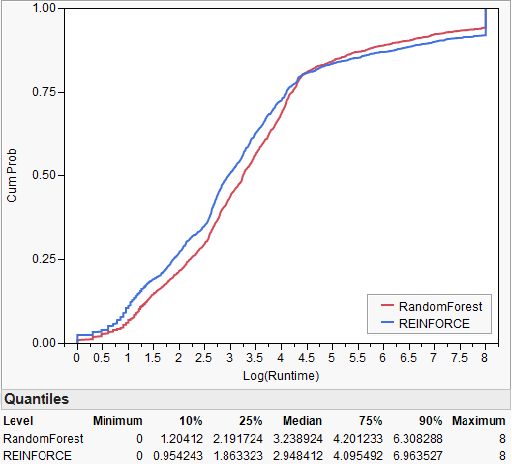
\includegraphics{./img/cdf.png}}
	\caption{Cumulative density plot of AS model performance}
	\label{fig:cdf}
\end{figure}
\chapter{Conclusion}
\section{Summary}
Given problem features and algorithm performance, an AS model can learn how to map problems to algorithms through supervised learning techniques, such as classification or regression algorithms. This makes sense because AS involves modelling the relationship between two variables: problem features and algorithm performance. However, it is also possible to consider an AS model as a decision-making entity: it \textit{senses} the problem features, \textit{decides} which algorithm to choose, \textit{observes} the performance of the chosen algorithm, and then \textit{updates} its decision-making behavior based on the observed response. This portrays a type of learning based on \textit{feedback} --– the core concept behind RL. Its primary advantage is that learning is not dependent on right-wrong examples explicitly labeled by a "teacher" as with supervised learning techniques; thus enabling an AS model to learn on its own based only on its observation of how algorithms behave with respect to problem features. It is more difficult to control the behavior of RL algorithms compared to supervised learning techniques, but when successful, an RL-trained AS model has far better learning generalization capability than one trained using supervised learning. Better generalization means better AS performance with previously unseen problems despite learning only from a small batch of problems.

Two AS models were implemented in this study: one trained using PRFR, a supervised learning technique used on a previous AS study by \citet{kotthoff2016portfolios}, and the other trained using REINFORCE, the RL algorithm proposed in this study. The AS models were compared using mean misclassification penalty (MCP), a performance metric which reflects the additional time required in solving problems where suboptimal algorithms were selected. A mean MCP of 0 indicates that there is zero penalty in choosing a suboptimal algorithm, signifying that the best algorithm is always selected for every problem. PRFR garnered an MCP of $6.22 \times 10^5$ milliseconds while REINFORCE measured 4x as worse, with mean MCP of $2.32 \times 10^{6}$ milliseconds. On the other hand, median performance results show that REINFORCE did better than PRFR on the easier problems on the dataset, representing 75\% of the total. Still, PRFR outperformed REINFORCE because it specialized in solving the much harder problems (problems solvable within $10^5-10^8$ ms range) which have a huge impact on MCP computation, despite representing a minority on the dataset.    


\section{Recommendations for Future Work}
A number of modifications on the REINFORCE algorithm can be explored:

\begin{itemize}
	\item Reduce number of input features \\ \\
	Only a handful of features might be necessary to perform effective AS. Dimensionality reduction methods (e.g. PCA, clustering) can help to reduce and simplify the problem feature space. This can assist a function approximator in focusing on few important features to learn algorithm scores.
	
	\item Redesign policy function and function approximator \\ \\
	The behavior of the policy function depends on how the function approximator calibrates the algorithm scores for each problem instance. In turn, the function approximator learns the proper calibrations when the policy allows for balanced \textit{exploration} and \textit{exploitation} during AS: \textit{explore} seldomly tried algorithms to learn their performance and \textit{exploit} existing knowledge on algorithm performance to select the best algorithm.
	
	It is quite difficult to know which function approximation technique goes best with a given policy function (and vice versa). This can be determined through cycles of reviewing the literature to get ideas which methods might potentially work and heavy experimentation. 
	
	\item Reward scaling \\ \\
	How the algorithm runtime is scaled prior to performance gradient calculation has a huge impact on the resulting performance of the AS model. Unscaled runtime values can serve enough as feedback; however, learning becomes more erratic especially when there are plenty of outliers across runtime observations. Reward scaling helps to stabilize learning. The optimum scaling method can be empirically determined, taking into consideration the characteristics of runtime data distribution and the function approximation method used.  
	
	\item Add regularization term to performance gradient \\ \\
	A regularization term acts as an offset value to the performance gradient which can influence how the policy function conducts \textit{exploration} and \textit{exploitation} among available actions. Gradient regularization methods such as entropy regularization (Williams, 1992) and importance sampling (Nachum et. al., 2016) attempt to improve exploration, which helps the policy to avoid being stuck with known actions and incentivize behavior towards discovery of potentially better actions. 
	
	\item Implement curriculum learning \\ \\
	A training strategy can be implemented such that problem instances are presented to the AS model in some meaningful order instead of being random. Such strategy is called \textit{curriculum learning} \citep{bengio2009curriculum}. This recommendation is based from the experiment results where REINFORCE performed well only on the easier problems but not on the harder ones. It might be possible to improve AS model performance by focusing the training on much harder problems. 	
\end{itemize}

Besides REINFORCE, there are plenty of other policy-gradient RL algorithms that can possibly be applied to AS. Another class of RL algorithms called \textit{contextual bandits} can also be explored. Contextual bandits assume a simpler model of RL where reward values are fully received for every input instead of being delayed across a series of inputs. This model can also apply to AS since algorithm performance is based only from the algorithm currently selected and not on past nor future algorithm choices.





\bibliographystyle{utmthesis-authordate}
\bibliography{reference}


\end{document}